\section{A hardware study on an IBM Heron processor}\label{sec:hardware}

The simulation study tests \qtrace{} against a twin whose honest noise we wrote ourselves. A hardware experiment tests the parts of the method that do not depend on optical physics, namely calibration against a device's own commissioning data, false-alarm control under real noise and drift, the value of tests that use the full outcome table, and agreement with information-theoretic predictions, on a device whose noise is not generated by any model of ours. It also makes the eavesdropper physical: her interaction is a unitary acting on the transmitted qubit and her own ancilla, and her information can be measured.

\subsection{Multiplexed BB84 links and physical eavesdroppers}\label{sec:hw-design}

Each BB84 link uses two neighbouring qubits: a data qubit that carries Alice's state to Bob's measurement and an ancilla owned by Eve. Pairs are ranked by two-qubit-gate error plus both readout errors, subject to cut-offs of 2\,\% and 5\,\% respectively, and are chosen mutually non-adjacent so that no coupler connects qubits of different links. On \HwBackend{} this gave \HwLinks{} links; \cref{tab:hwcal} in \cref{app:hardware} summarises their calibration. One circuit realises one BB84 round per link and per shot (\cref{fig:circuit}). The eight settings $(a,\alpha,\beta)$ rotate in a Latin-square pattern, link $i$ in circuit $c$ using setting $(i+c)\bmod 8$, so that every circuit contains every setting and every link sees every setting once per pass of eight circuits.

\begin{figure}[!tbp]
\centering
\begin{quantikz}[row sep=0.35cm, column sep=0.32cm, font=\small]
\lstick{data: $\ket{0}$} & \gate{X^{a}} & \gate{H^{\alpha}} & \slice{} & \gate[2]{U_{\rm Eve}} & \slice{} & \gate{H^{\beta}} & \meter{} & \setwiretype{c} \rstick{Bob}\\
\lstick{ancilla: $\ket{0}$} & & & & & & \gate{(HS^\dagger)^{y}} & \meter{} & \setwiretype{c} \rstick{Eve}
\end{quantikz}
\caption{One BB84 link. Alice prepares $\ket{a}$ in basis $\alpha$; Eve applies $U_{\rm Eve}\in\{\mathbb{1},\,R_{ZX}(\theta),\,R_{XX}(\theta),\,U_{\rm AD}(\gamma)\}$; Bob measures in basis $\beta$. Eve's ancilla is read in the $Y$ basis ($y=1$) for the entangling probes and in the $Z$ basis for the damping probe. Barriers (dashed) align all links of a circuit.}
\label{fig:circuit}
\end{figure}

The experiment comprises two commissioning passes, in which every link is honest, followed by six monitoring epochs of one pass each. In the monitoring epochs every link is honest in two epochs and attacked in four, with four distinct probes drawn from a balanced, seeded schedule. Ten probes are used.

\paragraph{Entangling probe.} Eve couples her ancilla to the data qubit with $R_{ZX}(\theta)=\exp(-i\theta Z\otimes X/2)$, which learns the $Z$-basis bit, or with $R_{XX}(\theta)=\exp(-i\theta X\otimes X/2)$, which learns the $X$-basis bit. For a data qubit in an eigenstate of the coupled Pauli operator with eigenvalue $(-1)^a$, the ancilla evolves to
\begin{equation}
\ket{e_\pm}=\cos\tfrac{\theta}{2}\ket{0}\mp i\sin\tfrac{\theta}{2}\ket{1},\qquad \braket{e_+}{e_-}=\cos\theta. \label{eq:probestates}
\end{equation}
A data qubit prepared in the conjugate basis becomes entangled with the ancilla, and its coherence is multiplied by $\braket{e_+}{e_-}$, so that Bob's error probability in the conjugate basis is
\begin{equation}
D(\theta)=\frac{1-\cos\theta}{2}=\sin^2\frac{\theta}{2}. \label{eq:disturb}
\end{equation}
Eve's optimal guess of the bit in the coupled basis is the Helstrom measurement \cite{Helstrom1976} discriminating $\ket{e_+}$ from $\ket{e_-}$, whose error probability is
\begin{equation}
P_{\rm err}(\theta)=\tfrac12\Bigl(1-\sqrt{1-\lvert\braket{e_+}{e_-}\rvert^2}\Bigr)=\frac{1-\sin\theta}{2}, \label{eq:helstrom}
\end{equation}
attained by a $Y$-basis measurement. Her information per bit in the coupled basis is $I(\theta)=1-\h\bigl(P_{\rm err}(\theta)\bigr)$. Eliminating $\theta$ with $\sin\theta=2\sqrt{D(1-D)}$ gives
\begin{equation}
I(D)=1-\h\!\Bigl(\tfrac12-\sqrt{D(1-D)}\Bigr), \label{eq:infodisturb}
\end{equation}
which has the same functional form as the optimal information--disturbance trade-off for individual attacks on BB84 derived by Fuchs \emph{et al.} \cite{Fuchs1997}. At $\theta=\pi/2$ the ancilla states are orthogonal and the probe is an intercept--resend attack in the coupled basis. Eve's choice between $R_{ZX}$ and $R_{XX}$ is balanced so that, in every pass, she matches Alice's basis on exactly half of the sifted settings; the average sifted QBER increase is then $\Delta Q_{\rm ideal}=\tfrac12\sin^2(\theta/2)$. A purely random choice per circuit would leave a probability of $1/16$ that an epoch is never disturbed, which a noisy rehearsal of the experiment revealed and which the balanced schedule removes.

\paragraph{Amplitude-damping probe.} The coupling $U_{\rm AD}(\gamma)=\mathrm{CX}_{e\to d}\,\mathrm{CR}_Y(2\arcsin\sqrt\gamma)_{d\to e}$ transfers the excitation of the data qubit to the ancilla with probability $\gamma$. It produces bit-asymmetric errors, $\gamma$ for $a=1$ and none for $a=0$ in the $Z$ basis and $(1-\sqrt{1-\gamma})/2$ in the $X$ basis, the qubit analogue of an efficiency-mismatch attack. Eve's ancilla is $\ket{1}$ only after a decay, so her information about $Z$-basis bits is $\h(\gamma/2)-\tfrac12\h(\gamma)$.

\paragraph{Execution.} All circuits were transpiled with a fixed layout and no routing, executed with the Qiskit Runtime sampler \cite{Qiskit2024} without error mitigation, twirling or dynamical decoupling (the monitor must work on raw device statistics), and with per-shot readout so that detection could later be studied as a function of the number of rounds. A pilot job of eight circuits with 400 shots measured the cost per shot (\HwPilotSec\,s); the main job of 64 circuits with \HwShots{} shots each used \HwMainSec\,s, a total of \HwTotalSec\,s of processor time for \HwRounds{} million link-rounds. Before any processor time was spent, the full pipeline was validated on a noisy simulation of the device.

\subsection{Tests}\label{sec:hw-tests}

For every link and monitoring epoch three tests compare the epoch with a reference. \emph{\qtrace{}} transfers the structure of the simulation monitor to the qubit setting: an error channel (two-sided change of the $Z$- and $X$-basis error rates, $\chi^2_2$), an asymmetry channel (change of $P(1\mid a=0)-P(0\mid a=1)$ per basis, $\chi^2_2$) and an omnibus channel (two-sample likelihood-ratio test over all eight settings, $\chi^2_8$), combined with a Bonferroni correction. The \emph{pooled QBER} test is the one-sided two-proportion test on the sifted QBER that deployed systems use; the \emph{per-basis QBER} test applies one-sided tests to both bases with a Bonferroni correction. Dispersion factors for between-circuit fluctuations were estimated from the two commissioning passes and were close to one ($\phi=\HwPhi$ for the omnibus channel, $\phi=\HwPhiQ$ for the pooled QBER), confirming that circuits repeat at the shot-noise level.

\subsection{Pre-registered analysis: the reference matters}\label{sec:hw-pre}

The analysis plan fixed before the run used the two commissioning passes as reference. With this reference every test failed: \qtrace{}, the per-basis QBER test and the pooled QBER test flagged \HwPreFAQT\,\%, \HwPreFAQB\,\% and \HwPreFAQP\,\% of the \HwHonestN{} honest link-epochs at $\alpha=10^{-3}$ (\cref{tab:hwpre} in \cref{app:hardware}). The cause is physical and is shown in \cref{fig:shift}. Relative to commissioning, the honest monitoring epochs show a QBER increase of \HwShiftX\,\% in the $X$ basis, on all \HwShiftXPos{} links, and of only \HwShiftZ\,\% in the $Z$ basis. The two commissioning passes agree to $\HwPassDiff$, and the increase shows no trend over the six epochs, so slow drift is excluded. Commissioning circuits contain no probe gates, so their qubits are measured immediately after preparation; in monitoring circuits the barriers make every data qubit, including those of honest links, wait for the longest probe on the chip, while two-qubit gates act on other links. A dephasing-dominated error that appears only under these conditions is what one expects from the added idle time together with crosstalk from concurrent coupler activation. The present data cannot separate the two contributions.

\begin{figure}[!tbp]
\centering
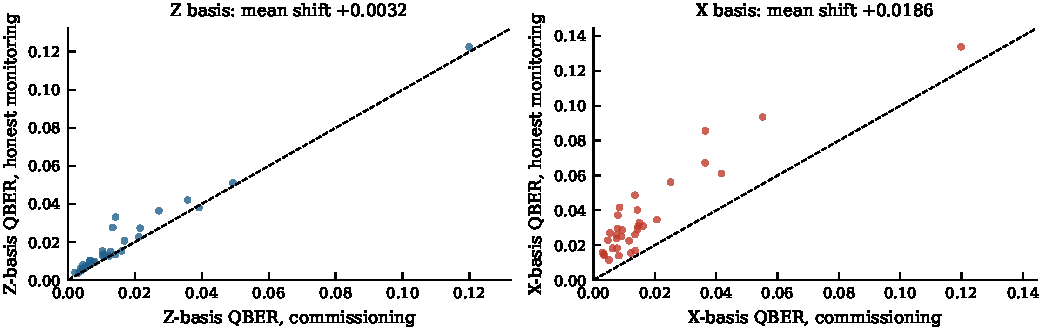
\includegraphics[width=\textwidth]{figures/hw_condition_shift.pdf}
\caption{Honest links on \HwBackend{}: QBER in the commissioning passes against QBER in the honest monitoring epochs, per basis. The $X$ basis shifts by \HwShiftX\,\% on every link, the $Z$ basis by \HwShiftZ\,\%: commissioning circuits did not reproduce the operating conditions of monitoring circuits.}
\label{fig:shift}
\end{figure}

The monitors were right. The operating conditions had changed, and a reference acquired under different conditions describes a different device. The same failure would occur in an optical system calibrated without traffic, with different detector gating, or at a different temperature. The practical lesson is that the commissioning data of any telemetry monitor, QBER-based or otherwise, must be acquired under the operating conditions of the monitored traffic; in the hardware setting this means inserting timing-matched delays and the same concurrent gate activity into the commissioning circuits.

\subsection{Condition-matched analysis}\label{sec:hw-matched}

Each link was honest in two monitoring epochs that ran under exactly the conditions of the attacked epochs. Using these epochs as reference, we test each attacked epoch against the link's two honest epochs and estimate the false-alarm rate by testing each honest epoch against the link's other honest epoch. This analysis was defined after the pre-registered one had failed and is reported as such.

With the condition-matched reference none of the \HwHonestN{} honest link-epochs was flagged by any test (\cref{tab:hwmatched}). The honest $p$-values are, if anything, conservative: 3\,\% fall below 0.05. The measured QBER increase of every entangling probe agrees with $\Delta Q_{\rm ideal}$ across two decades (\cref{fig:hwphys}a); for example $\theta=0.60$ gives \HwThetaDMeas\,\% against \HwThetaDIdeal\,\% predicted and $\theta=0.90$ gives \HwThetaEMeas\,\% against \HwThetaEIdeal\,\%. The damping probe raises the QBER above its ideal value at small $\gamma$, because its three two-qubit gates add their own error, an honest feature of a physical eavesdropper whose apparatus is imperfect.

\begin{table}[!tbp]
\centering
\caption{Hardware detection with the condition-matched reference: fraction of link-epochs flagged at $\alpha=10^{-3}$; $n$ is the number of link-epochs, $\Delta Q_{\rm ideal}$ the ideal and $\Delta Q_{\rm meas}$ the measured increase of the sifted QBER.}
\label{tab:hwmatched}
\small
\begin{tabular}{lccccccc}
\toprule
Probe & $n$ & $\Delta Q_{\rm ideal}$ (\%) & $\Delta Q_{\rm meas}$ (\%) & Q-TRACE & QBER/basis & QBER pooled & Omnibus \\
\midrule
Honest (no probe) & 66 & 0.00 & 0.00 & 0.00 & 0.00 & 0.00 & 0.00 \\
\midrule
$\theta=0.15$ & 14 & 0.28 & 0.49 & 1.00 & 0.93 & 0.64 & 1.00 \\
$\theta=0.25$ & 13 & 0.78 & 0.87 & 0.92 & 0.85 & 0.85 & 0.92 \\
$\theta=0.40$ & 14 & 1.97 & 2.11 & 1.00 & 1.00 & 1.00 & 1.00 \\
$\theta=0.60$ & 14 & 4.37 & 4.34 & 1.00 & 1.00 & 1.00 & 1.00 \\
$\theta=0.90$ & 13 & 9.46 & 9.05 & 1.00 & 1.00 & 1.00 & 1.00 \\
$\theta=1.57$ & 13 & 25.00 & 23.10 & 1.00 & 1.00 & 1.00 & 1.00 \\
\midrule
$\gamma=0.03$ & 13 & 1.13 & 2.82 & 1.00 & 1.00 & 1.00 & 1.00 \\
$\gamma=0.06$ & 12 & 2.26 & 3.49 & 1.00 & 1.00 & 1.00 & 1.00 \\
$\gamma=0.12$ & 12 & 4.55 & 5.99 & 1.00 & 1.00 & 1.00 & 1.00 \\
$\gamma=0.25$ & 14 & 9.60 & 10.05 & 1.00 & 1.00 & 1.00 & 1.00 \\
\bottomrule
\end{tabular}

\end{table}

All probes with $\Delta Q_{\rm ideal}\ge 2$\,\% are detected on every link-epoch by every test. The informative case is the weakest probe, $\theta=0.15$, with $\Delta Q_{\rm ideal}=\HwThetaAIdeal$\,\%: \qtrace{} flags \HwThetaAQT{} of \HwThetaAN{} link-epochs, the per-basis QBER test \HwThetaAQB{} and the pooled QBER test \HwThetaAQP. The pooled test loses power because the probe disturbs one basis at a time and pooling dilutes the signal. The per-basis test is close to optimal here, since on qubits almost every disturbance is a change of an error rate; \qtrace{} matches it while retaining channels for asymmetric and unsifted deviations.

\begin{figure}[!tbp]
\centering
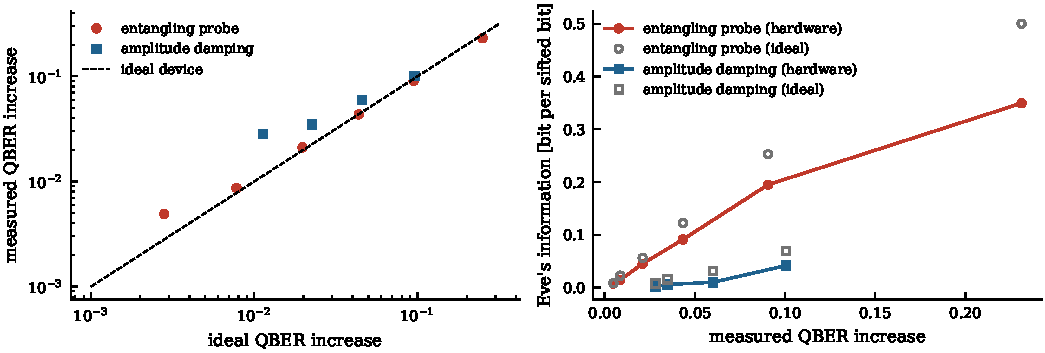
\includegraphics[width=\textwidth]{figures/hw_physics.pdf}
\caption{Probe physics on \HwBackend{} (condition-matched reference). (a) Measured against ideal increase of the sifted QBER; the dashed line is the ideal device. (b) Eve's information per sifted bit, measured on her ancilla, against the measured QBER increase; open symbols are the ideal-device values of \cref{eq:infodisturb} and of the damping channel.}
\label{fig:hwphys}
\end{figure}

\subsection{Rounds to detection and information leaked before the alarm}\label{sec:hw-info}

Because every shot was recorded, detection can be studied as a function of the number of rounds by subsampling the shots of the tested epoch. \Cref{fig:rounds} shows the detection probability against shots per circuit for the three weakest probes, and \cref{tab:hwleak} the number of shots per circuit at which half of the attacked link-epochs are flagged. For $\theta=0.15$, \qtrace{} needs \HwShotsWeakQT{} shots, the per-basis test \HwShotsWeakQB{} and the pooled QBER test \HwShotsWeakQP, a factor of \HwShotsRatio{} more. The omnibus channel alone would need \HwShotsWeakOM.

\begin{figure}[!tbp]
\centering
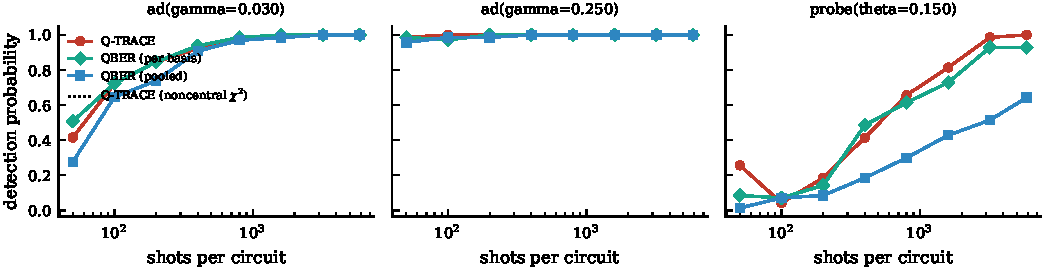
\includegraphics[width=\textwidth]{figures/hw_rounds.pdf}
\caption{Detection probability at $\alpha=10^{-3}$ against the number of shots per circuit of the tested epoch, for the three weakest probes on \HwBackend{} (condition-matched reference; mean over five random subsamples per point).}
\label{fig:rounds}
\end{figure}

Eve's ancilla measurements turn this into an operational quantity. On sifted rounds in which her probe basis matched Alice's basis, her measured information agrees with \cref{eq:infodisturb} up to the effect of her own readout errors (\cref{fig:hwphys}b and \cref{tab:hwinfo}); for $\theta=0.40$ it is \HwInfoFourMeas{} bit against \HwInfoFourIdeal{} ideally, and for the intercept--resend limit $\theta=\pi/2$ it is \HwIRInfo{} bit with a guessing error of \HwIRGuess. Multiplying the information per sifted bit by the number of sifted rounds needed for detection gives the information Eve gathers before the median first alarm: for $\theta=0.15$ this is \HwLeakWeakQT{} bits under \qtrace{}, \HwLeakWeakQB{} bits under the per-basis QBER test and \HwLeakWeakQP{} bits under the pooled QBER monitor. These are small numbers in absolute terms; their ratio is what transfers to a deployed system, where the same reasoning applies per window.
